\section{Monofilare Helixantenne}
Die Helixantenne ist die in der Satellitenkommunikationstechnik die am Weitesten verbreitete Antennenart \cite{HelicalAntennas}. Der Grund hierfür ist die Immunität der zirkularen Polarisation gegenüber Faraday Rotation. Dieses Phänomen findet in der Ionosphäre statt \cite{FaradayRotation} und wurde in (REFERENZ) bereits näher erklärt.

Die Helixantenne hat weiters verschiedene Operationsmodi. Arbeitet die Antenne im Normal-Modus, so zeigt sie ein omnidirektionales Abstrahlverhalten, wobei sie senkrecht zur Achse der Antenne gleichmäßig in alle Richtungen strahlt. Dieser Betriebsmodus wird erreicht, sobald der Umfang einer Windung der Helix im Vergleich zu der Wellenlänge $\lambda=\frac{c}{f}$ klein ist. Der zweite Modus der Wendelantenne ist der Axial-Modus. Befindet sich die Antenne in diesem Betriebsverhalten, so verändert sich die Richtung der Strahlung. Der Großteil der elektromagnetischen Strahlung wird nun entlang der Achse der Spirale abgegeben. Dieser Modus wird erreicht, sobald die Wellenlänge ungefähr gleich groß ist wie der Umfang einer Windung der Spirale \cite{HelicalAntennas}.

Da die Wendelantenne über eine besonders große Bandbreite verfügt, eignet sie sich gut für den Nachbau. Hierbei sind der Durchmesser sowie die Steigung der Spirale von ausschlaggebender Relevanz für die gewünschte Einsatzfrequenz. Der Durchmesser für eine Wendelantenne im Axial-Modus ist hierbei mit $D=\frac{\lambda}{\pi}$ definiert. Die Stromverteilung auf der Helix ergibt sich folglich wie in Abbildung \ref{fig:CrntDis-Helix} ersichtlich. \cite{HelicalAntennas}.

\begin{figure}[H]
	\centering
	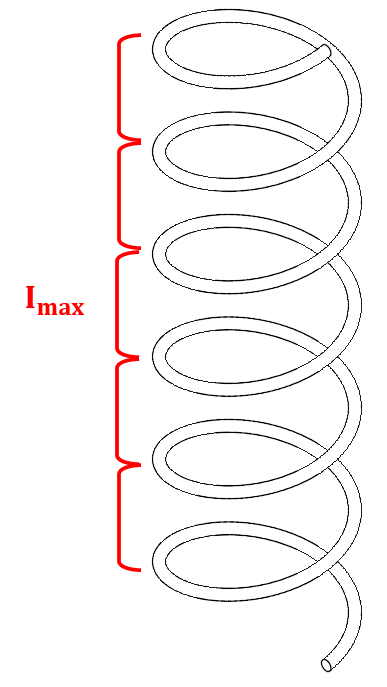
\includegraphics[width=4cm]{../ref/Spirale_Doku}
	\caption{Stromverteilung auf einer Helix-Antenne}
	\label{fig:CrntDis-Helix}
\end{figure}

Ein Richtwert für die Steigung der Helix ergibt sich empirisch mit einem Steigungswinkel zwischen 12° und 14° \cite{helixWebsite}. Die Steigung der Spirale ist so wichtig für die Funktionalität der Antenne, da sie sich mit einem größeren Winkel eher wie ein Dipol verhält, und mit einem kleineren Winkel eher wie eine Ringantenne. REFERENZ

Die folgenden Bezeichnungen werden zur Beschreibung der Helix verwendet.
\begin{itemize}
	\item D: Durchmesser der Helix
	\item S: Abstand zwischen den einzelnen Windungen
	\item U: Umfang der Helix
	\item $\alpha$: Steigung der Helix
	\item L: Länge einer Windung
	\item n: Anzahl der Windungen
	\item Lges: Gesamtlänge der Helix
	\item d: Durchmesser des Leiters
\end{itemize}

Um den Winkel zu berechnen, lässt sich die aufgerollte Windung der Helix betrachten (Abbildung \ref{fig:Wndg_aufgerollt}).

\begin{figure}[H]
	\centering
	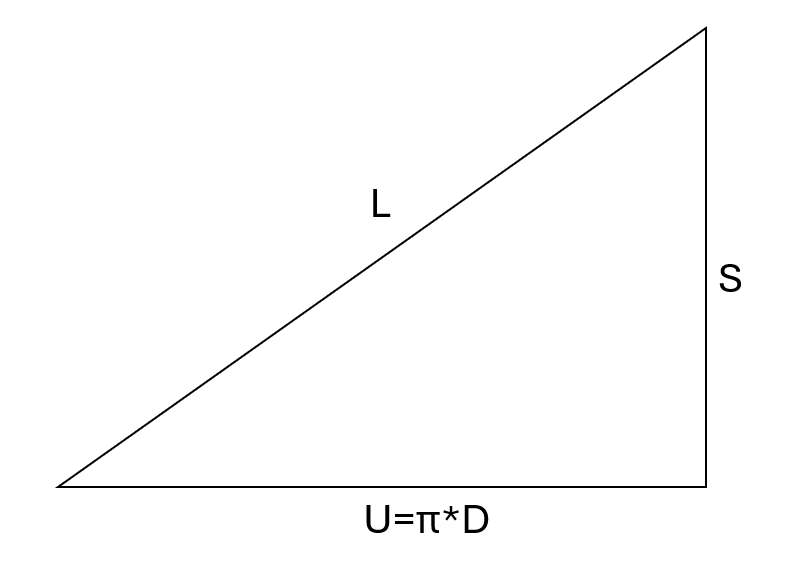
\includegraphics[width=6cm]{../ref/Windung_aufgerollt.png}
	\label{fig:Wndg_aufgerollt}
\end{figure}

Hier lässt sich ein rechtwinkliges Dreieck erkennen. Die Ankathete ist hierbei der Umfang einer Windung und die Gegenkathete stellt den Abstand zwischen den einzelnen Drehungen dar. Somit lässt sich der Winkel $\alpha$ mit der Formel

\begin{equation}
	\alpha=\arctan(\frac{S}{C})
\end{equation}

beschreiben. Ein weiterer vitaler Parameter für die Funktionalität der Antenne ist der Abstand zwischen den einzelnen Windungen. Dieser wird generell für $0,23\lambda$ als ideal angegeben. MISSING REFERENCE

Der Reflektor kann verschiedene Formen annehmen. Er kann kreisförmig, viereckig oder auch trichterförmig sein. Für die Zwecke dieser Diplomarbeit wurde ein kreisförmiger Reflektor gewählt. Als passend wird hierbei ein Durchmesser von $\frac{3\lambda}{4}$ angesehen. Der Durchmesser des Leiters ist unkritisch für die Funktion der Antenne, allerdings wird als Richtwert ein Querschnitt von $0,005\lambda$ bis $0,05\lambda$ als passend betrachtet. 

Nachfolgend sind die wichtigsten Gleichungen für die Berechnung der Parameter einer Helix-Antenne gegeben \cite{Kraus-2002-AntennasB}.

\begin{table}[H]
	\begin{tabular}{|l|l|}

		\textbf{Bezeichnung} & \textbf{Formel}\\ 
		benötigte Kabellänge & $L=n*\sqrt{\lambda^2+S^2}$ \\
		D				     & $D=\frac{\lambda}{\pi}$\\ 
		Halbwertsbreite		 & $HPBW=\frac{52}{C*\sqrt{nS}}$ \\ 
		Gewinn               & $G=12*C^2nS$                 \\ 
		Eingangsimpedanz     & $Z=\frac{150}{\sqrt{C}}$      \\ 
		Effektive Apertur    & $Ae=\frac{D*\lambda^2}{4*\pi}$ \\ 
		\end{tabular}
	\end{table}

Der Antennengewinn der Helix wächst mit jeder hinzugefügten Windung an. Dieser ist als

\begin{equation}
	G=12*C^2nS
\end{equation}

definiert \cite{helix-calc-daycounter}. Es lässt sich hierbei die Windungsanzahl $"$n$"$ erkennen, die den Gewinn direkt proportional anwachsen lässt. Eine weitere wichtige Kenngröße von Antennen ist die Halbwertsbreite. Diese lässt sich mit

\begin{equation}
	HPBW=\frac{52}{C*\sqrt{nS}}
\end{equation}

ermitteln.

\subsection{Funktionsweise und charakteristische Eigenschaften}
Dipol/Ringantenne Zusammenhang erklären, zirkulare Polarisation, Zusammenhang mit der Stromverteilung, Erklärung des Abstandes zwischen den Windungen, Durchmesser, Reflektor erklären,
